\begin{figure}[H]
	\center
	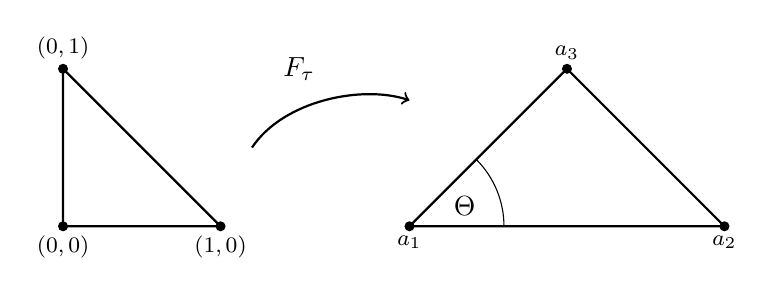
\begin{tikzpicture}[scale=2]

	% first simplix
	\draw[thick] (0,0) -- ++(0,1) -- ++(1,-1)--cycle;
	\filldraw (0,0)         circle (0.8pt);
	\filldraw (0,0) ++(1,0) circle (0.8pt);
	\filldraw (0,0) ++(0,1) circle (0.8pt);
	\fill[black,font=\footnotesize] (0,0) node[below] {$(0,0)$}
									(0,0) ++(1,0) node[below] {$(1,0)$}
									(0,0) ++(0,1) node[above] {$(0,1)$};
	
	%arrow
	\draw[thick,-to] (1.2,0.5) .. controls (1.4,0.8) and (1.9,0.9) .. (2.2, 0.8);
	
	%second simplex							
	\draw[thick] (2.2,0) -- ++(2,0) -- ++(-1,1)--cycle;
	\filldraw (2.2,0)         circle (0.8pt);
	\filldraw (2.2,0) ++(2,0) circle (0.8pt);
	\filldraw (2.2,0) ++(1,1) circle (0.8pt);
	\fill[black,font=\footnotesize] (2.2,0) node[below] {$a_1$}
									(2.2,0) ++(2,0) node[below] {$a_2$}
									(2.2,0) ++(1,1) node[above] {$a_3$};								
								
	
%	\pgfmathsetmacro{\ax}{2.2}
%	\pgfmathsetmacro{\ay}{0}
	
	\draw (2.2,0) ++(45:.6) arc (45:0:.6);
								
																		
	\node at (1.5,1) {$F_{\tau}$};
	\node at (2.55,0.13) {$\Theta$};				
	

	\end{tikzpicture}
		
	\caption{affine transformation}
	\label{ch1_plot_affin_equiv_triang}

\end{figure}